\tableofcontents
\section*{Предисловие}
При выполнении данной лабораторной работы было решено использовать 
\href{https://python-control.readthedocs.io/en/0.9.4/}{Python Control Systems Library}.
Данный инструмент является альтернативой Matlab, адаптированной для использования на 
языке Python и предоставляет широкий функционал для анализа и моделирования систем,
а также синтеза регуляторов для управления.

Полный листинг моделирования систем представлен в \href{https://github.com/diuzhevVlad/control-theory-itmo-fall-2023/blob/main/Lab7/Lab7.ipynb}{jupyter notebook} на GitHub.

\pagebreak


\section{Полностью управляемая система}
Рассмотрим систему, заданную матрицами $A$ и $B$:
\begin{equation*}
    A = \begin{bmatrix}
        7 & -7 & 8 \\
        6 & -5 & 6 \\
        -6 & 4 & -7
    \end{bmatrix},
    B = \begin{bmatrix}
        -4 \\ -2 \\ 4
    \end{bmatrix}
\end{equation*}

\subsection{Матрица управляемости}
Запишем матрицу управляемости системы:
\begin{equation*}
    U = \begin{bmatrix}
        B & AB & A^2B 
    \end{bmatrix}
     = 
    \begin{bmatrix}
        -4 & 18 & -40 \\
        -2 & 10 & -14 \\
        4 & -12 & 16
    \end{bmatrix}
\end{equation*}
Заметим, что ранг данной матрицы равен 3, следовательно, система - полностью управляема.

\subsection{Жорданова форма}
Представим систему в Жордановом базисе:
\begin{equation}
    \begin{cases}
        \dot{\hat{x}} = P^{-1}AP\hat{x} + P^{-1}Bu  \\
        y = CP\hat{x}
    \end{cases}
\end{equation}
где $P$ - матрица обобщенных векторов. ЖНФ матрицы $A$:
\begin{equation*}
    A = PJP^{-1} = \begin{bmatrix}
        -1 & -\frac{3}{2} + \frac{i}{2} & -\frac{3}{2}-\frac{i}{2} \\
        0 & -1 & -1 \\
        1 & 1 & 1
    \end{bmatrix}
    \begin{bmatrix}
        -1 & 0 & 0 \\
        0 & -2-3i & 0 \\
        0 & 0 & -2+3i
    \end{bmatrix}
    \begin{bmatrix}
        -1 & -\frac{3}{2} + \frac{i}{2} & -\frac{3}{2}-\frac{i}{2} \\
        0 & -1 & -1 \\
        1 & 1 & 1
    \end{bmatrix}^{-1}
\end{equation*}
Матрица входных воздействий в Жордановом базисе:
\begin{equation*}
    P^{-1}B = \begin{bmatrix}
        2 \\ 1-i \\ 1+i
    \end{bmatrix}
\end{equation*}
Все жордановы клетки матрицы $J$ соответсвуют разным собственным числам и элементы матрицы входных воздействий
соответствующие концам клеток не равны нулю. Следовательно: все собственные чила - управляемы.

Также, заметим:
\begin{equation*}
    \begin{cases}
        rank(\begin{bmatrix}
            A - (-1)\cdot I &  B
        \end{bmatrix} ) = 3 \\
        rank(\begin{bmatrix}
            A - (-2-3i)\cdot I &  B
        \end{bmatrix} ) = 3 \\
        rank(\begin{bmatrix}
            A - (-2+3i)\cdot I &  B
        \end{bmatrix} ) = 3
    \end{cases}
\end{equation*}
что подтверждает управляемость всех собственных чисел.

\subsection{Управляемое подпространство}
Т.к. система - полностью управляема, управляемое подпространство совпадает с $\mathcal{R}^3$ и любой вектор
принадлежит ему, в том числе $x_1$:
\begin{equation*}
    x_1 = \begin{bmatrix}
        5 \\
        3 \\
        -3
    \end{bmatrix}
\end{equation*}

\subsection{Грамиан управляемости}
Расчитаем грамиан управляемости системы:
\begin{equation}
    P(t_1) = \int_{0}^{t_1}e^{At}BB^Te^{A^Tt}dt
\end{equation}
\begin{equation*}
    P(3) = \begin{bmatrix}
        1.777 & 0.654 & -1.982 \\
        0.654 & 0.538 & -0.538 \\
        -1.982 & -0.539 & 2.534
        \end{bmatrix}
\end{equation*}
Собственные числа грамиана:
\begin{eqnarray*}
    \lambda_1 = 0.055, \lambda_2 = 0.439, \lambda_3 = 4.355
\end{eqnarray*}

\subsection{Расчет управления}
Расчитаем управление, необходимое для перехода из нулевого состояния в состояние $x_1$ за $t_1$ секунд:
\begin{equation}
    u(t) = B^Te^{A^T(t_1-t)}(P(t_1))^{-1}x_1
\end{equation}
Искомое управление:
\begin{equation*}
    u(t) = B^Te^{A^T(3-t)}(P(3))^{-1}x_1 = -9.196e^{t-3} - 32.765e^{2t-6}sin(3t-9)-5.244e^{2t-6}cos(3t-9)
\end{equation*}

\subsection{Моделирование}
Выполним моделирование системы. Можем видеть, что система достагла желаемого состояния.
\begin{figure}[h]
    \centering
    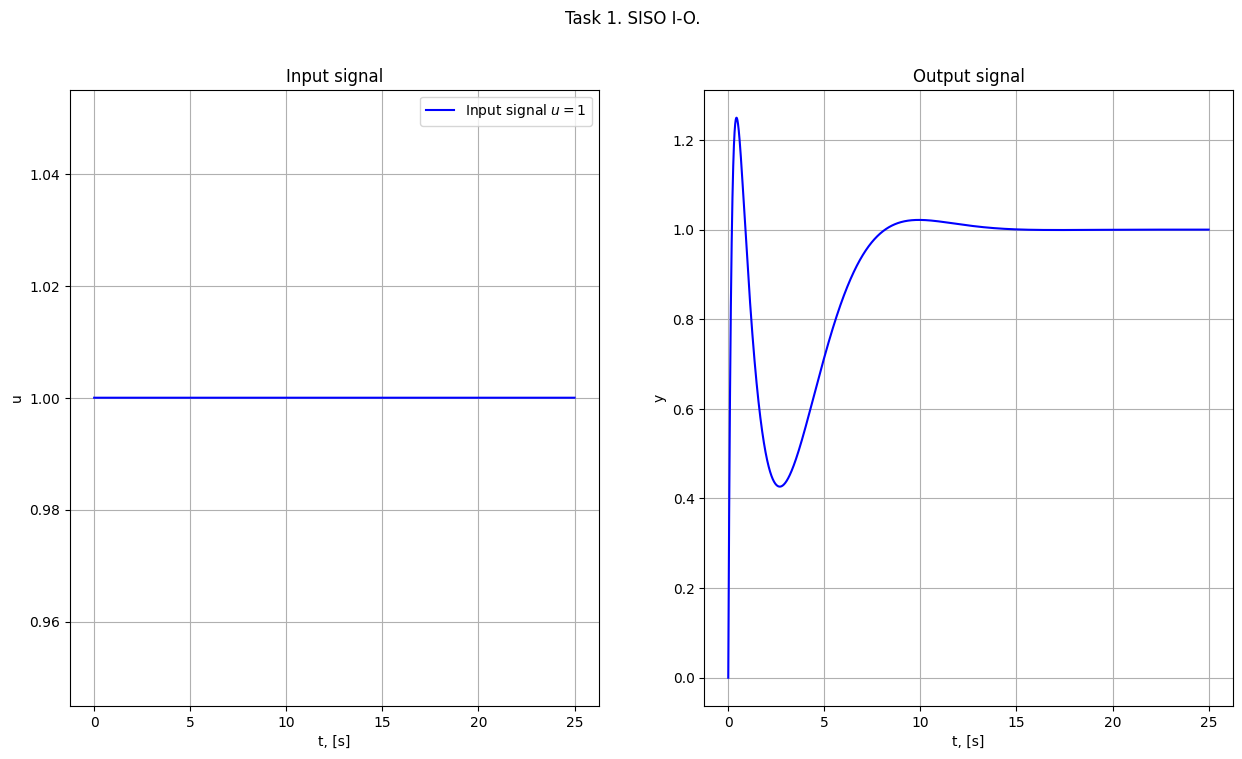
\includegraphics[width=\textwidth]{plot_1_1.png}
    \caption{\label{fig:The-caption-1}Задание 1. Компоненты вектра состояний при расчитаном управлении}
\end{figure}

\begin{figure}[]
    \centering
    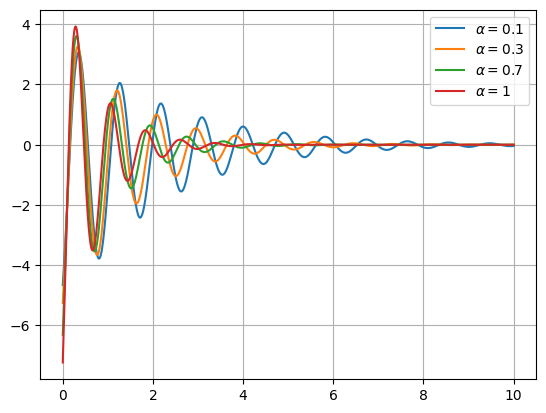
\includegraphics[width=\textwidth]{plot_1_2.png}
    \caption{\label{fig:The-caption-1}Задание 1. Расчитанное управляющее воздействие}
\end{figure}
\pagebreak

\section{Частично управляемая система}
Рассмотрим систему, заданную матрицами $A$ и $B$:
\begin{equation*}
    A = \begin{bmatrix}
        7 & -7 & 8 \\
        6 & -5 & 6 \\
        -6 & 4 & -7
    \end{bmatrix},
    B = \begin{bmatrix}
        2 \\ 0 \\ 0
    \end{bmatrix}
\end{equation*}

\subsection{Матрица управляемости}
Запишем матрицй управляемости системы:
\begin{equation*}
    U = \begin{bmatrix}
        B & AB & A^2B 
    \end{bmatrix}
     = 
    \begin{bmatrix}
        2 & 14 & -82 \\
        0 & 12 & -48 \\
        0 & -12 & 48
    \end{bmatrix}
\end{equation*}
Заметим, что ранг данной матрицы равен 2, следовательно, система - частично управляема.

\subsection{Жорданова форма}
Представление системы в Жордановом базисе идентично заданию 1.
Матрица входных воздействий в Жордановом базисе:
\begin{equation*}
    P^{-1}B = \begin{bmatrix}
        0 \\ -2i \\ 2i
    \end{bmatrix}
\end{equation*}
Все жордановы клетки матрицы $J$ соответсвуют разным собственным числам, однако элемент матрицы входных воздействий
соответствующий концу клетки -1 равен нулю. Следовательно: собственное число -1 - неуправляемо.

Также, заметим:
\begin{equation*}
    \begin{cases}
        rank(\begin{bmatrix}
            A - (-1)\cdot I &  B
        \end{bmatrix} ) = 2 \\
        rank(\begin{bmatrix}
            A - (-2-3i)\cdot I &  B
        \end{bmatrix} ) = 3 \\
        rank(\begin{bmatrix}
            A - (-2+3i)\cdot I &  B
        \end{bmatrix} ) = 3
    \end{cases}
\end{equation*}
что подтверждает прошлый вывод.

\subsection{Управляемое подпространство}
\begin{equation*}
    x_1' = \begin{bmatrix}
        5 \\
        3 \\
        -3
    \end{bmatrix},
    x_1'' = \begin{bmatrix}
        4 \\
        3 \\
        -2
    \end{bmatrix}
\end{equation*}
\begin{equation*}
    \begin{cases}
        rank(\begin{bmatrix}
            U &  x_1'
        \end{bmatrix} ) = 2 \\
        rank(\begin{bmatrix}
            U &  x_1''
        \end{bmatrix} ) = 3 \\
    \end{cases}
\end{equation*}
Можем сделать вывод, что вектор $x_1'$ лежит в управляемом подпространстве.

\subsection{Грамиан управляемости}
Расчитаем грамиан управляемости системы:
\begin{equation*}
    P(3) = \begin{bmatrix}
        5.153 & 2.538 & -2.538 \\
        2.538 & 1.385 & -1.385 \\
        -2.538 & -1.385 & 1.385
        \end{bmatrix}
\end{equation*}
Собственные числа грамиана:
\begin{eqnarray*}
    \lambda_1 = 7.744, \lambda_2 = 0.179, \lambda_3 = 0
\end{eqnarray*}

\subsection{Расчет управления}
Расчитаем управление, необходимое для перехода из нулевого состояния в состояние $x_1$ за $t_1$ секунд:
\begin{equation}
    u(t) = B^Te^{A^T(t_1-t)}(P(t_1))^{\dagger}x_1
\end{equation}
Искомое управление:
\begin{equation*}
    u(t) = B^Te^{A^T(3-t)}(P(3))^{-1}x_1 = -10e^{2t-6}sin(3t-9) - 2e^{2t-6}cos(3t-9)
\end{equation*}

\subsection{Моделирование}
Выполним моделирование системы. Можем видеть, что система достагла желаемого состояния.
\begin{figure}[h]
    \centering
    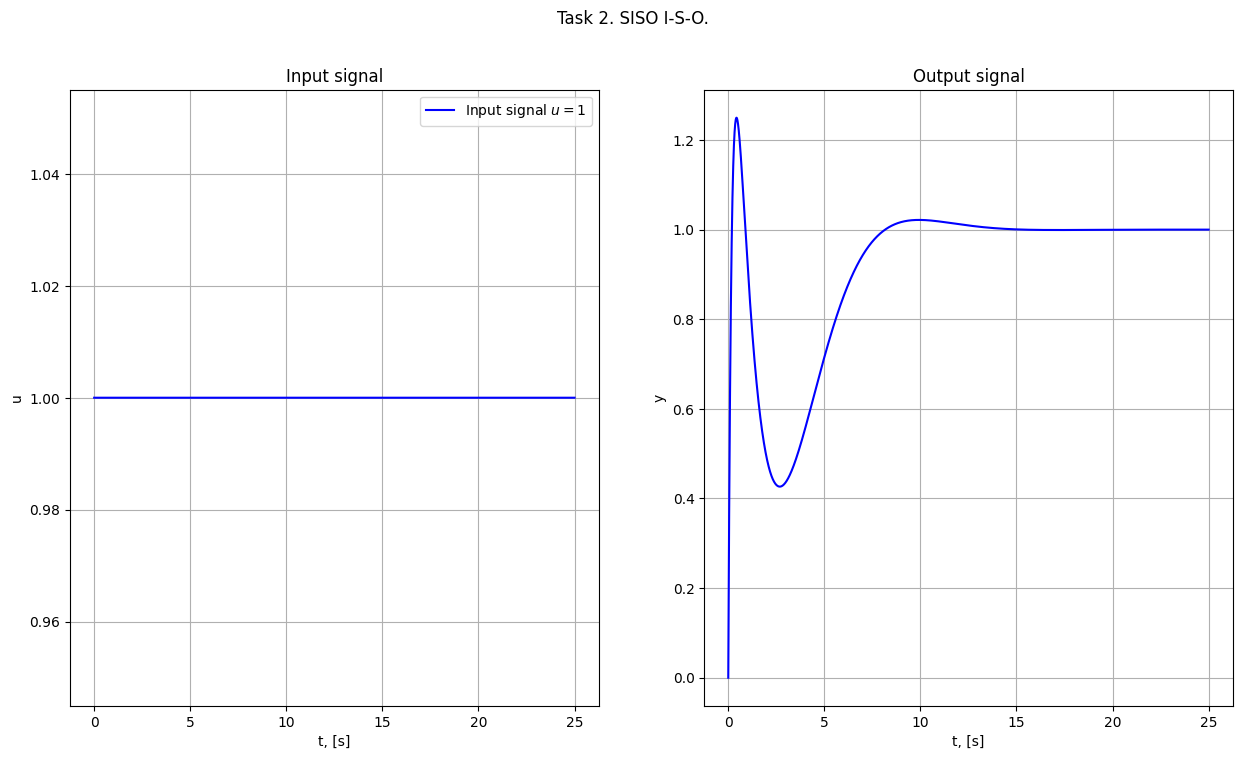
\includegraphics[width=\textwidth]{plot_2_1.png}
    \caption{\label{fig:The-caption-1}Задание 2. Компоненты вектра состояний при расчитаном управлении}
\end{figure}

\begin{figure}[]
    \centering
    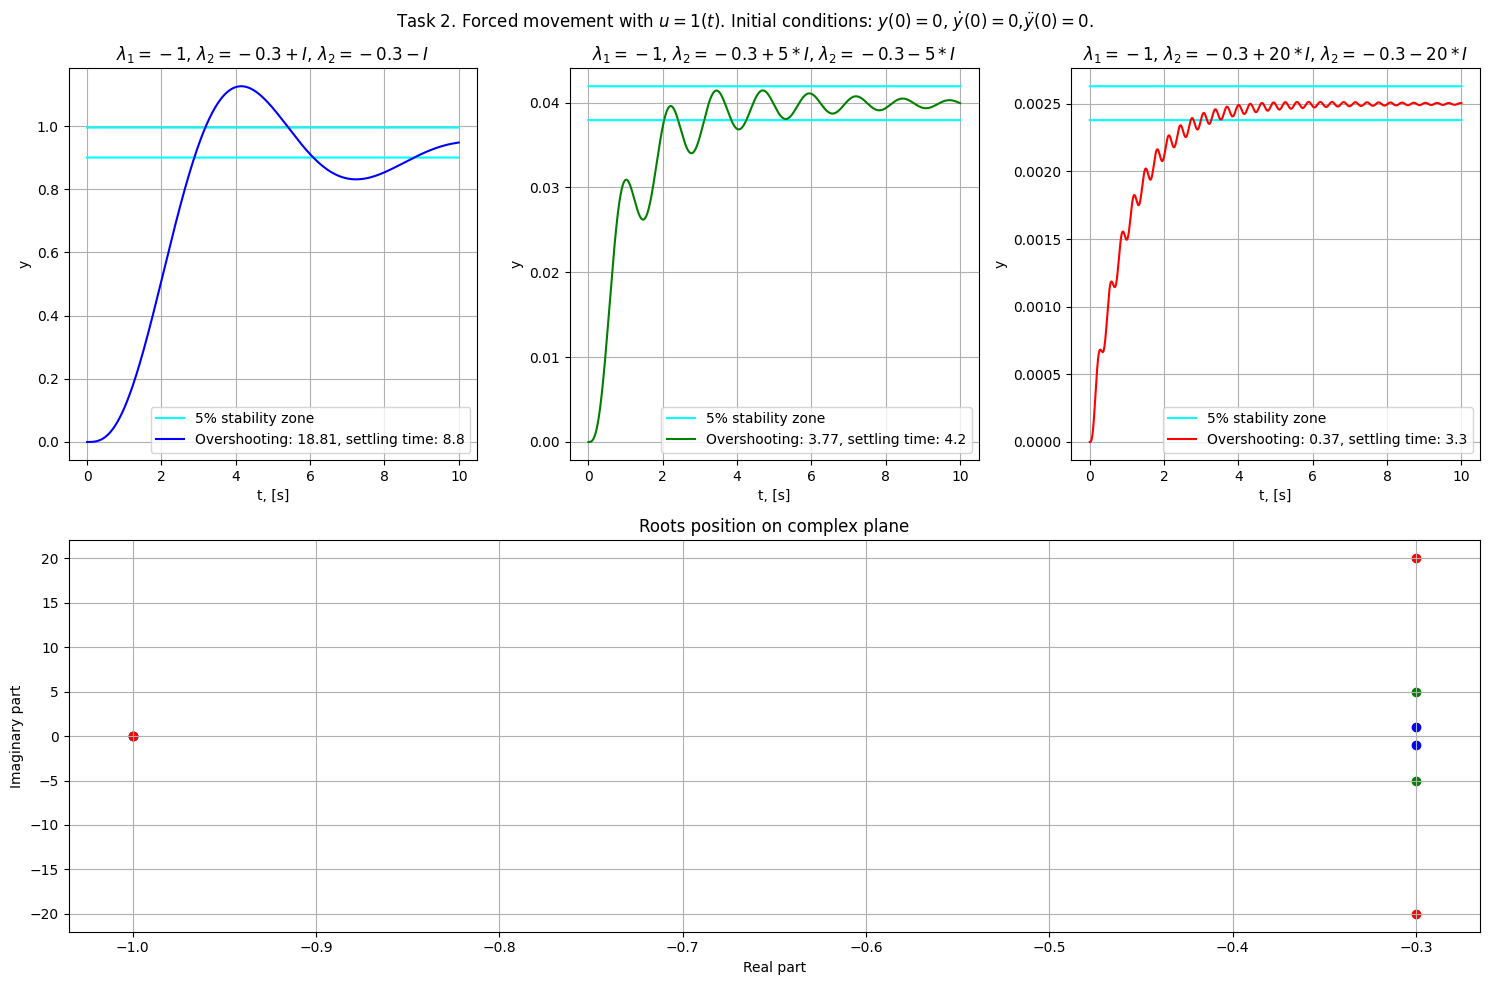
\includegraphics[width=\textwidth]{plot_2_2.png}
    \caption{\label{fig:The-caption-1}Задание 2. Расчитанное управляющее воздействие}
\end{figure}
\pagebreak

\section{Полностью наблюдаемая система}
Рассмотрим систему:
\begin{equation}
    \dot{x} = Ax, y = Cx
\end{equation}
\begin{equation*}
    A = \begin{bmatrix}
        -10 & 3 & -8 \\
        -5 & 0 & -6 \\
        6 & -4 & 3
    \end{bmatrix},
    C = \begin{bmatrix}
        2 & 1 & 5
    \end{bmatrix}
\end{equation*}

\subsection{Матрица наблюдаемости}
Запишем матрицу наблюдаемости системы:
\begin{equation*}
    V = \begin{bmatrix}
        C \\ CA \\ CA^2
    \end{bmatrix}
     = 
    \begin{bmatrix}
        2 & 1 & 5 \\
        5 & -14 & -7 \\
        -22 & 43 & 23
    \end{bmatrix}
\end{equation*}
Заметим, что ранг данной матрицы равен 3, следовательно, система - полностью наблюдаема.

\subsection{Жорданова форма}
Представим систему в Жордановом базисе. ЖНФ матрицы $A$:
\begin{equation*}
    A = PJP^{-1},
    J = \begin{bmatrix}
        1 & 0 & 0 \\
        0 & -4-i & 0 \\
        0 & 0 & -4+i
    \end{bmatrix}
\end{equation*}
Матрица выхода в Жордановом базисе:
\begin{equation*}
    CP = \begin{bmatrix}
        2 & \frac{3}{2}(1-i) & \frac{3}{2}(1+i)
    \end{bmatrix}
\end{equation*}
Все жордановы клетки матрицы $J$ соответсвуют разным собственным числам и элементы матрицы выхода
соответствующие началам клеток не равны нулю. Следовательно: все собственные чила - наблюдаемы.

Также, заметим:
\begin{equation*}
    \begin{cases}
        rank(\begin{bmatrix}
            A - (1)\cdot I \\  C
        \end{bmatrix} ) = 3 \\
        rank(\begin{bmatrix}
            A - (-4-i)\cdot I \\ C
        \end{bmatrix} ) = 3 \\
        rank(\begin{bmatrix}
            A - (-4+i)\cdot I \\ C
        \end{bmatrix} ) = 3
    \end{cases}
\end{equation*}
что подтверждает наблюдаемость всех собственных чисел.

\subsection{Грамиан наблюдаемости}
Расчитаем грамиан наблюдаемости системы:
\begin{equation}
    Q(t_1) = \int_{0}^{t_1}e^{A^Tt}C^TCe^{At}dt
\end{equation}
\begin{equation*}
    Q(3) = \begin{bmatrix}
        806.09 & -803.52 & 808.02 \\
        -803.52 & 802.35 & -804.23 \\
        808.02 & -804.23 & 811.05
        \end{bmatrix}
\end{equation*}
Собственные числа грамиана:
\begin{eqnarray*}
    \lambda_1 = 2.417, \lambda_2 = 0.002, \lambda_3 = 2.456
\end{eqnarray*}

\subsection{Расчет начальных условий}
Выходной сигнал системы:
\begin{equation*}
    y(t) = -3e^{-4t}cos(t) + 3e^{-4t}sin(t)
\end{equation*}
Расчитаем начальные условия для реализации данного выхода:
\begin{equation}
    x_0 = (Q(t_1))^{-1}\int_{0}^{t_1}e^{A^Tt}C^Ty(t)dt
\end{equation}
\begin{equation*}
    x_0 = \begin{bmatrix}
        3 \\ 1 \\ -2
    \end{bmatrix}
\end{equation*}

\subsection{Ненаблюдаемое подпространство}
Т.к. система является полностью наблюдаемой, по определению каждой траектории соответсвует один вектор начальных условий.

\subsection{Моделирование}
Выполним моделирование свободного движения системы при заданных начальных условиях:
\begin{figure}[h]
    \centering
    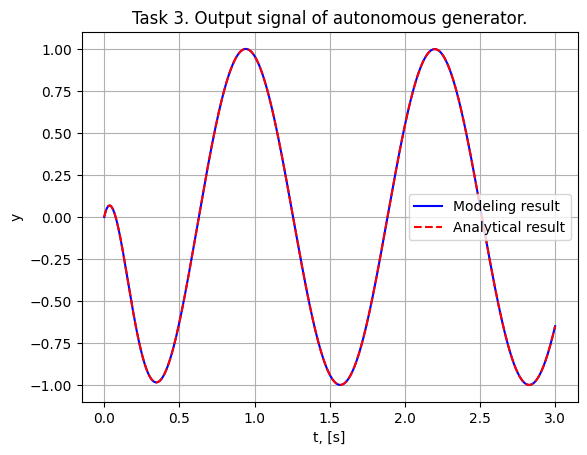
\includegraphics[width=\textwidth]{plot_3_1.png}
    \caption{\label{fig:The-caption-1}Задание 3. Компоненты вектра состояний при расчитаном управлении}
\end{figure}

\begin{figure}[]
    \centering
    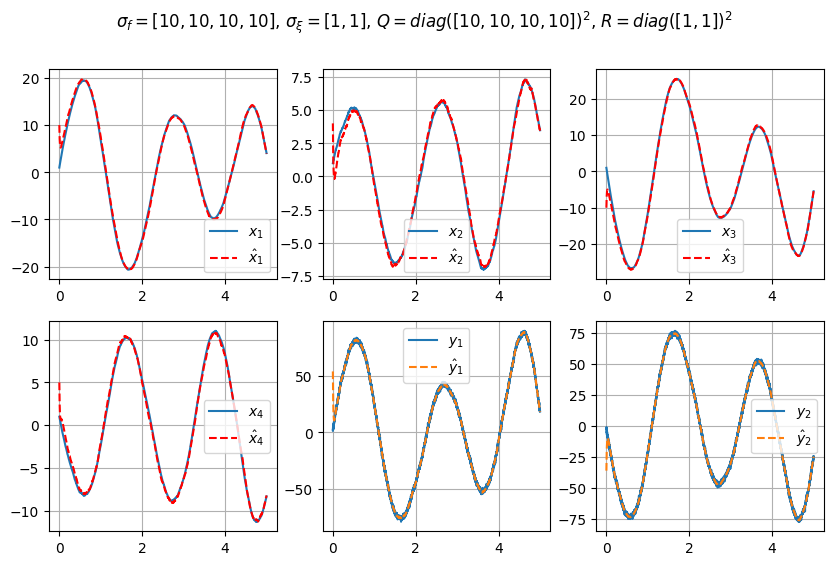
\includegraphics[width=\textwidth]{plot_3_2.png}
    \caption{\label{fig:The-caption-1}Задание 3. Сравнение выходного сигнала с желаемым}
\end{figure}
\pagebreak


\section{Частично наблюдаемая система}
Рассмотрим систему:
\begin{equation*}
    A = \begin{bmatrix}
        -10 & 3 & -8 \\
        -5 & 0 & -6 \\
        6 & -4 & 3
    \end{bmatrix},
    C = \begin{bmatrix}
        0 & 3 & 3
    \end{bmatrix}
\end{equation*}

\subsection{Матрица наблюдаемости}
Запишем матрицу наблюдаемости системы:
\begin{equation*}
    V = \begin{bmatrix}
        C \\ CA \\ CA^2
    \end{bmatrix}
     = 
    \begin{bmatrix}
        0 & 3 & 3 \\
        3 & -12 & -9 \\
        -24 & 45 & 21
    \end{bmatrix}
\end{equation*}
Заметим, что ранг данной матрицы равен 2, следовательно, система - частично наблюдаема.

\subsection{Жорданова форма}
Представим систему в Жордановом базисе. ЖНФ матрицы $A$:
\begin{equation*}
    A = PJP^{-1},
    J = \begin{bmatrix}
        1 & 0 & 0 \\
        0 & -4-i & 0 \\
        0 & 0 & -4+i
    \end{bmatrix}
\end{equation*}
Матрица выхода в Жордановом базисе:
\begin{equation*}
    CP = \begin{bmatrix}
        0 & \frac{3}{2}(1-i) & \frac{3}{2}(1+i)
    \end{bmatrix}
\end{equation*}
Все жордановы клетки матрицы $J$ соответсвуют разным собственным числам, однако элемент матрицы выхода 
соответствующие началу первой клетки равен нулю. Следовательно: собственное число 1 - ненаблюдаемо.

Также, заметим:
\begin{equation*}
    \begin{cases}
        rank(\begin{bmatrix}
            A - (1)\cdot I \\  C
        \end{bmatrix} ) = 2 \\
        rank(\begin{bmatrix}
            A - (-4-i)\cdot I \\ C
        \end{bmatrix} ) = 3 \\
        rank(\begin{bmatrix}
            A - (-4+i)\cdot I \\ C
        \end{bmatrix} ) = 3
    \end{cases}
\end{equation*}
что подтверждает прошлый вывод.

\subsection{Грамиан наблюдаемости}
Расчитаем грамиан наблюдаемости системы:
\begin{equation*}
    Q(3) = \begin{bmatrix}
        0.033 & 0.132 & 0.165 \\
        0.132 & 1.091 & 1.224 \\
        0.165 & 1.224 & 1.389
        \end{bmatrix}
\end{equation*}
Собственные числа грамиана:
\begin{eqnarray*}
    \lambda_1 = 2.492, \lambda_2 = 0.022, \lambda_3 = 0
\end{eqnarray*}

\subsection{Расчет начальных условий}
Выходной сигнал системы:
\begin{equation*}
    y(t) = -3e^{-4t}cos(t) + 3e^{-4t}sin(t)
\end{equation*}
Расчитаем начальные условия для реализации данного выхода:
\begin{equation}
    x_0 = (Q(t_1))^{\dagger}\int_{0}^{t_1}e^{A^Tt}C^Ty(t)dt
\end{equation}
\begin{equation*}
    x_0 = \begin{bmatrix}
        1 \\ -1 \\ 0
    \end{bmatrix}
\end{equation*}

\subsection{Ненаблюдаемое подпространство}
Любой вектор из ядра матрицы наблюдаемости является ненаблюдаемым и сложение любого вектора из него с вектором
начальных условий не повлияет на выход системы.
\begin{equation*}
    Nullspace(V) = \mathcal{L}(\begin{bmatrix}
        -1 & -1 & 1
    \end{bmatrix}^T)
\end{equation*}

\subsection{Моделирование}
Выполним моделирование свободного движения системы при заданных начальных условиях. Можем наблюдать, что во 
всех случаях желаемых выходной сигнал совпал с полученным в результате моделирования:
\begin{figure}[h]
    \centering
    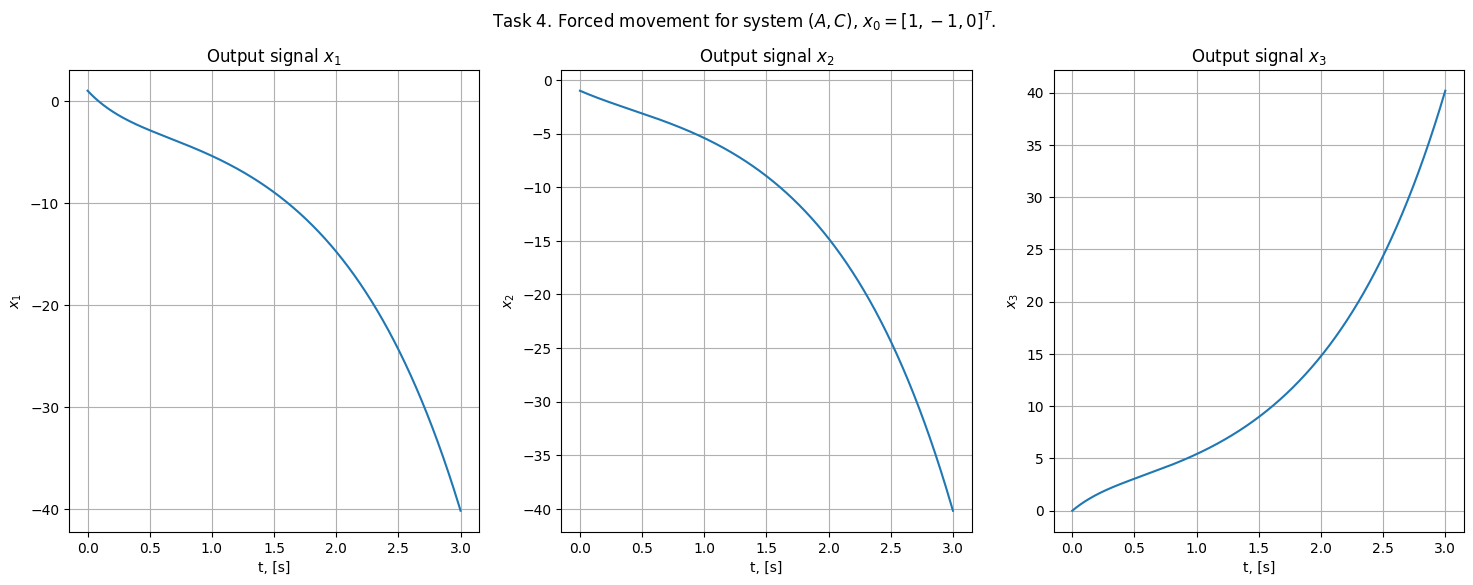
\includegraphics[width=\textwidth]{plot_4_1.png}
    \caption{\label{fig:The-caption-1}Задание 4. Компоненты вектра состояний при расчитаных начальных условиях (1)}
\end{figure}

\begin{figure}[]
    \centering
    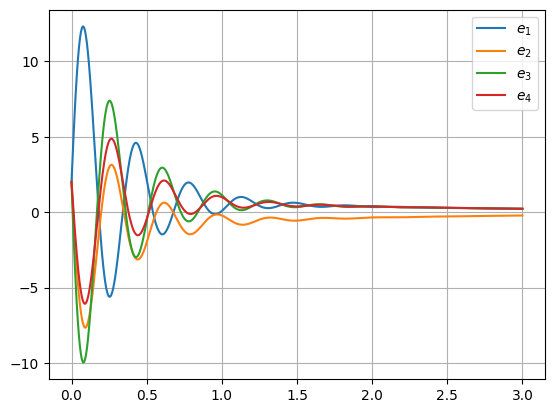
\includegraphics[width=\textwidth]{plot_4_2.png}
    \caption{\label{fig:The-caption-1}Задание 4. Сравнение выходного сигнала с желаемым (1)}
\end{figure}

\begin{figure}[]
    \centering
    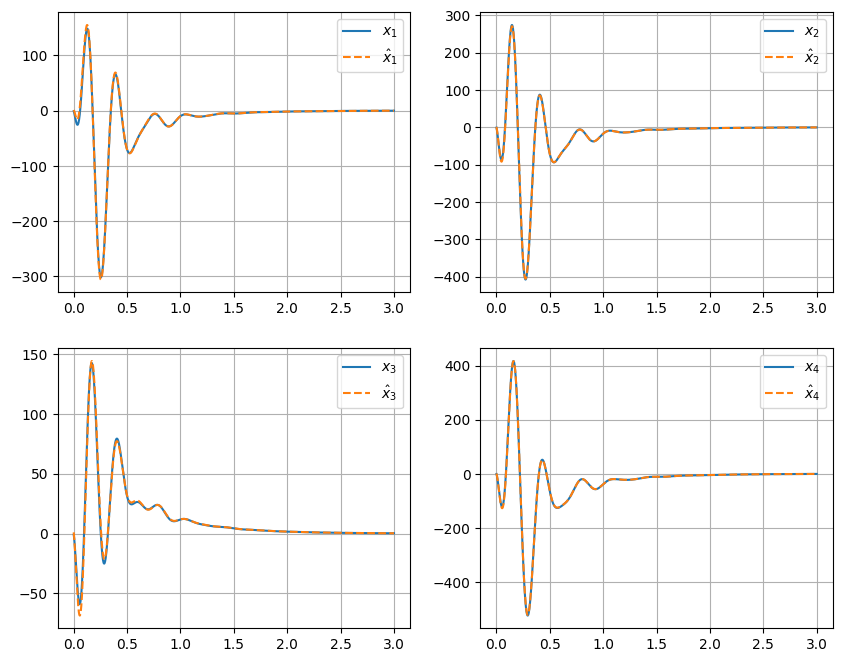
\includegraphics[width=\textwidth]{plot_4_3.png}
    \caption{\label{fig:The-caption-1}Задание 4. Компоненты вектра состояний при расчитаных начальных условиях (2)}
\end{figure}

\begin{figure}[]
    \centering
    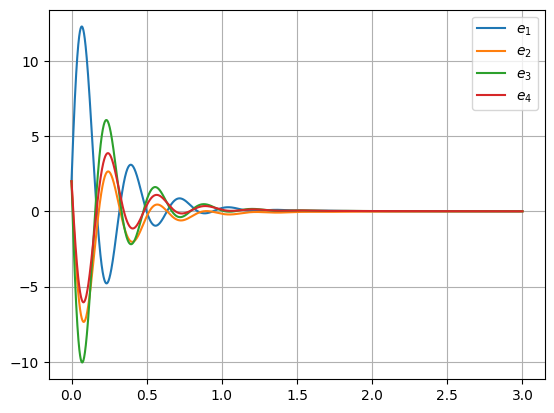
\includegraphics[width=\textwidth]{plot_4_4.png}
    \caption{\label{fig:The-caption-1}Задание 4. Сравнение выходного сигнала с желаемым (2)}
\end{figure}

\begin{figure}[]
    \centering
    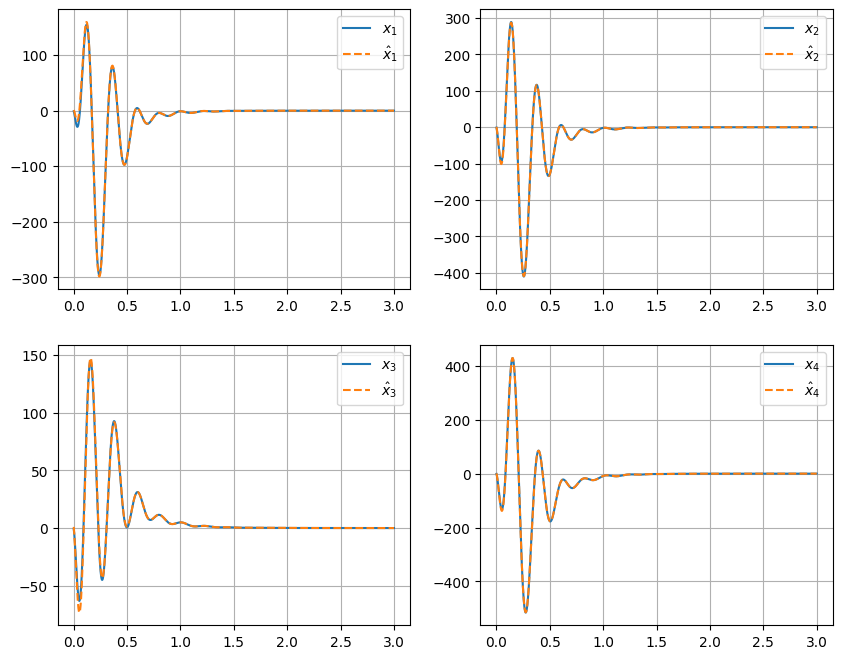
\includegraphics[width=\textwidth]{plot_4_5.png}
    \caption{\label{fig:The-caption-1}Задание 4. Компоненты вектра состояний при расчитаных начальных условиях (3)}
\end{figure}

\begin{figure}[]
    \centering
    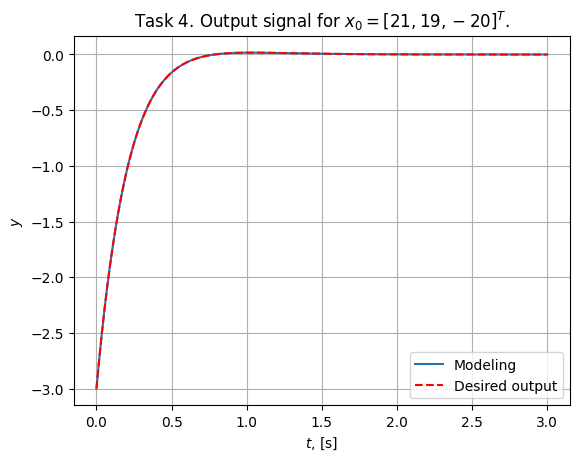
\includegraphics[width=\textwidth]{plot_4_6.png}
    \caption{\label{fig:The-caption-1}Задание 4. Сравнение выходного сигнала с желаемым (3)}
\end{figure}

\pagebreak

\section{Выводы}
В ходе выполнения работы удалось ознакомиться с понятиями управляемости и наблюдаемости, на практике исследовать
поведение управляемых и наблюдаемых систем и изучить их свойства.

Результаты моделирования подтверждают приведенные теоретические выкладки: расчитанное предложенным способом 
управление способно привести систему к желаемому состоянию, также удалось добиться желаемого выходного
сигнала заданием расчитанных начальных условий.